\section{Implementación}
\subsection{Arquitectura General}
La implementación se dividió en varios módulos con responsabilidades bien definidas, siguiendo principios de diseño orientado a objetos.
El sistema está compuesto por tres componentes principales:

\begin{enumerate}
    \item \textbf{Cliente (upload.py / download.py):} Aplicaciones CLI independientes
    \item \textbf{Servidor (start-server.py):} Servidor concurrente multi-thread
    \item \textbf{Librería RDT (lib/):} Módulos compartidos para el protocolo
\end{enumerate}

\subsection{Estructura de paquetes}
Todos los paquetes siguen una estructura de header fijo de 14 bytes seguido de un payload variable.

\begin{table}[H]
\centering
\begin{tabular}{@{}lll@{}}
\toprule
\textbf{Campo}        & \textbf{Tamaño} & \textbf{Descripción} \\ \midrule
\texttt{seq\_num}     & 1 byte  & Número de secuencia (0-255, con wrap-around) \\
\texttt{checksum}     & 1 byte  & Suma de verificación para detección de errores \\
\texttt{ack\_num}     & 1 byte  & Número de ACK (usado en paquetes ACK) \\
\texttt{payload\_length} & 4 bytes & Longitud del payload en bytes \\
\texttt{file\_size}   & 4 bytes & Tamaño total del archivo (solo en INIT) \\
\texttt{packet\_type} & 1 byte  & Tipo de paquete (ver tabla siguiente) \\
\texttt{protocol}     & 1 byte  & Protocolo utilizado (1=Stop\&Wait, 2=Selective Repeat) \\
\texttt{session\_id}  & 1 byte  & Identificador de sesión (1-255) \\ \bottomrule
\end{tabular}
\caption{Campos del Header (14 bytes)}
\end{table}

\subsection{Tipos de paquetes}
En el protocolo implementado, cada paquete tiene un tipo específico que determina su función dentro de la transferencia de archivos. A continuación se describen los tipos de paquetes utilizados y su propósito principal:

\begin{itemize}
    \item \textbf{DATA (1)}: Transferencia de datos, contiene los fragmentos del archivo.
    \item \textbf{ACK (2)}: Acknowledgment de paquetes DATA recibidos correctamente.
    \item \textbf{UPLOAD\_INIT (3)}: Inicia una sesión de subida (upload) de archivo.
    \item \textbf{DOWNLOAD\_INIT (4)}: Inicia una sesión de descarga (download) de archivo.
    \item \textbf{ACCEPT (5)}: Acepta la transferencia en respuesta a un paquete INIT.
    \item \textbf{ACCEPT\_ACK (6)}: Confirma la finalización del handshake.
    \item \textbf{FIN (7)}: Indica la finalización de la transferencia de datos.
    \item \textbf{FIN\_ACK (8)}: Confirma la finalización de la sesión.
    \item \textbf{ERROR (9)}: Mensaje de error, enviado por el servidor ante problemas o rechazos.
\end{itemize}

\begin{table}[H]

\label{tab:packet_types}
\renewcommand{\arraystretch}{2}
\begin{tabularx}{\textwidth}{|>{\centering\arraybackslash}m{3cm}|p{3cm}|X|X|}
\hline
\textbf{Tipo} & \textbf{Dirección} & \textbf{Payload} & \textbf{Campos Relevantes} \\ \hline

\textbf{UPLOAD
\_INIT (3)}
& Cliente $\rightarrow$ Servidor
& Nombre del archivo (UTF-8)
& \texttt{file\_size} (bytes), \texttt{protocol}, \texttt{session\_id=0} \\ \hline

\textbf{DOWNLOAD
\_INIT (4)}
& Cliente $\rightarrow$ Servidor
& Nombre del archivo (UTF-8)
& \texttt{file\_size=0}, \texttt{protocol}, \texttt{session\_id=0} \\ \hline

\textbf{ACCEPT (5)}
& Servidor $\rightarrow$ Cliente
& Puerto dedicado en ASCII (ej: ``52341'') o vacío
& \texttt{session\_id} (1–255 asignado) \\ \hline

\textbf{ACCEPT
\_ACK (6)}
& Cliente $\rightarrow$ Servidor
& Vacío
& \texttt{session\_id}, \texttt{ack\_num=0} \\ \hline

\textbf{DATA (1)}
& Bidireccional
& Fragmento de archivo (hasta 4096 bytes)
& \texttt{seq\_num}, \texttt{session\_id}, \texttt{payload\_length} \\ \hline

\textbf{ACK (2)}
& Receptor $\rightarrow$ Emisor
& Vacío
& \texttt{ack\_num}, \texttt{session\_id} \\ \hline

\textbf{FIN (7)}
& Emisor $\rightarrow$ Receptor
& Vacío
& \texttt{session\_id} \\ \hline

\textbf{FIN\_ACK (8)}
& Receptor $\rightarrow$ Emisor
& Vacío
& \texttt{session\_id} \\ \hline

\textbf{ERROR (9)}
& Servidor $\rightarrow$ Cliente
& Mensaje de error en UTF-8
& Texto descriptivo (ej: ``File not found'') \\ \hline

\end{tabularx}
\centering
\caption{Tipos de Paquetes del Protocolo}
\end{table}

\subsection{Flujos del Protocolo}
\subsubsection{Handshake (upload)}

\begin{figure}[H]
    \centering
    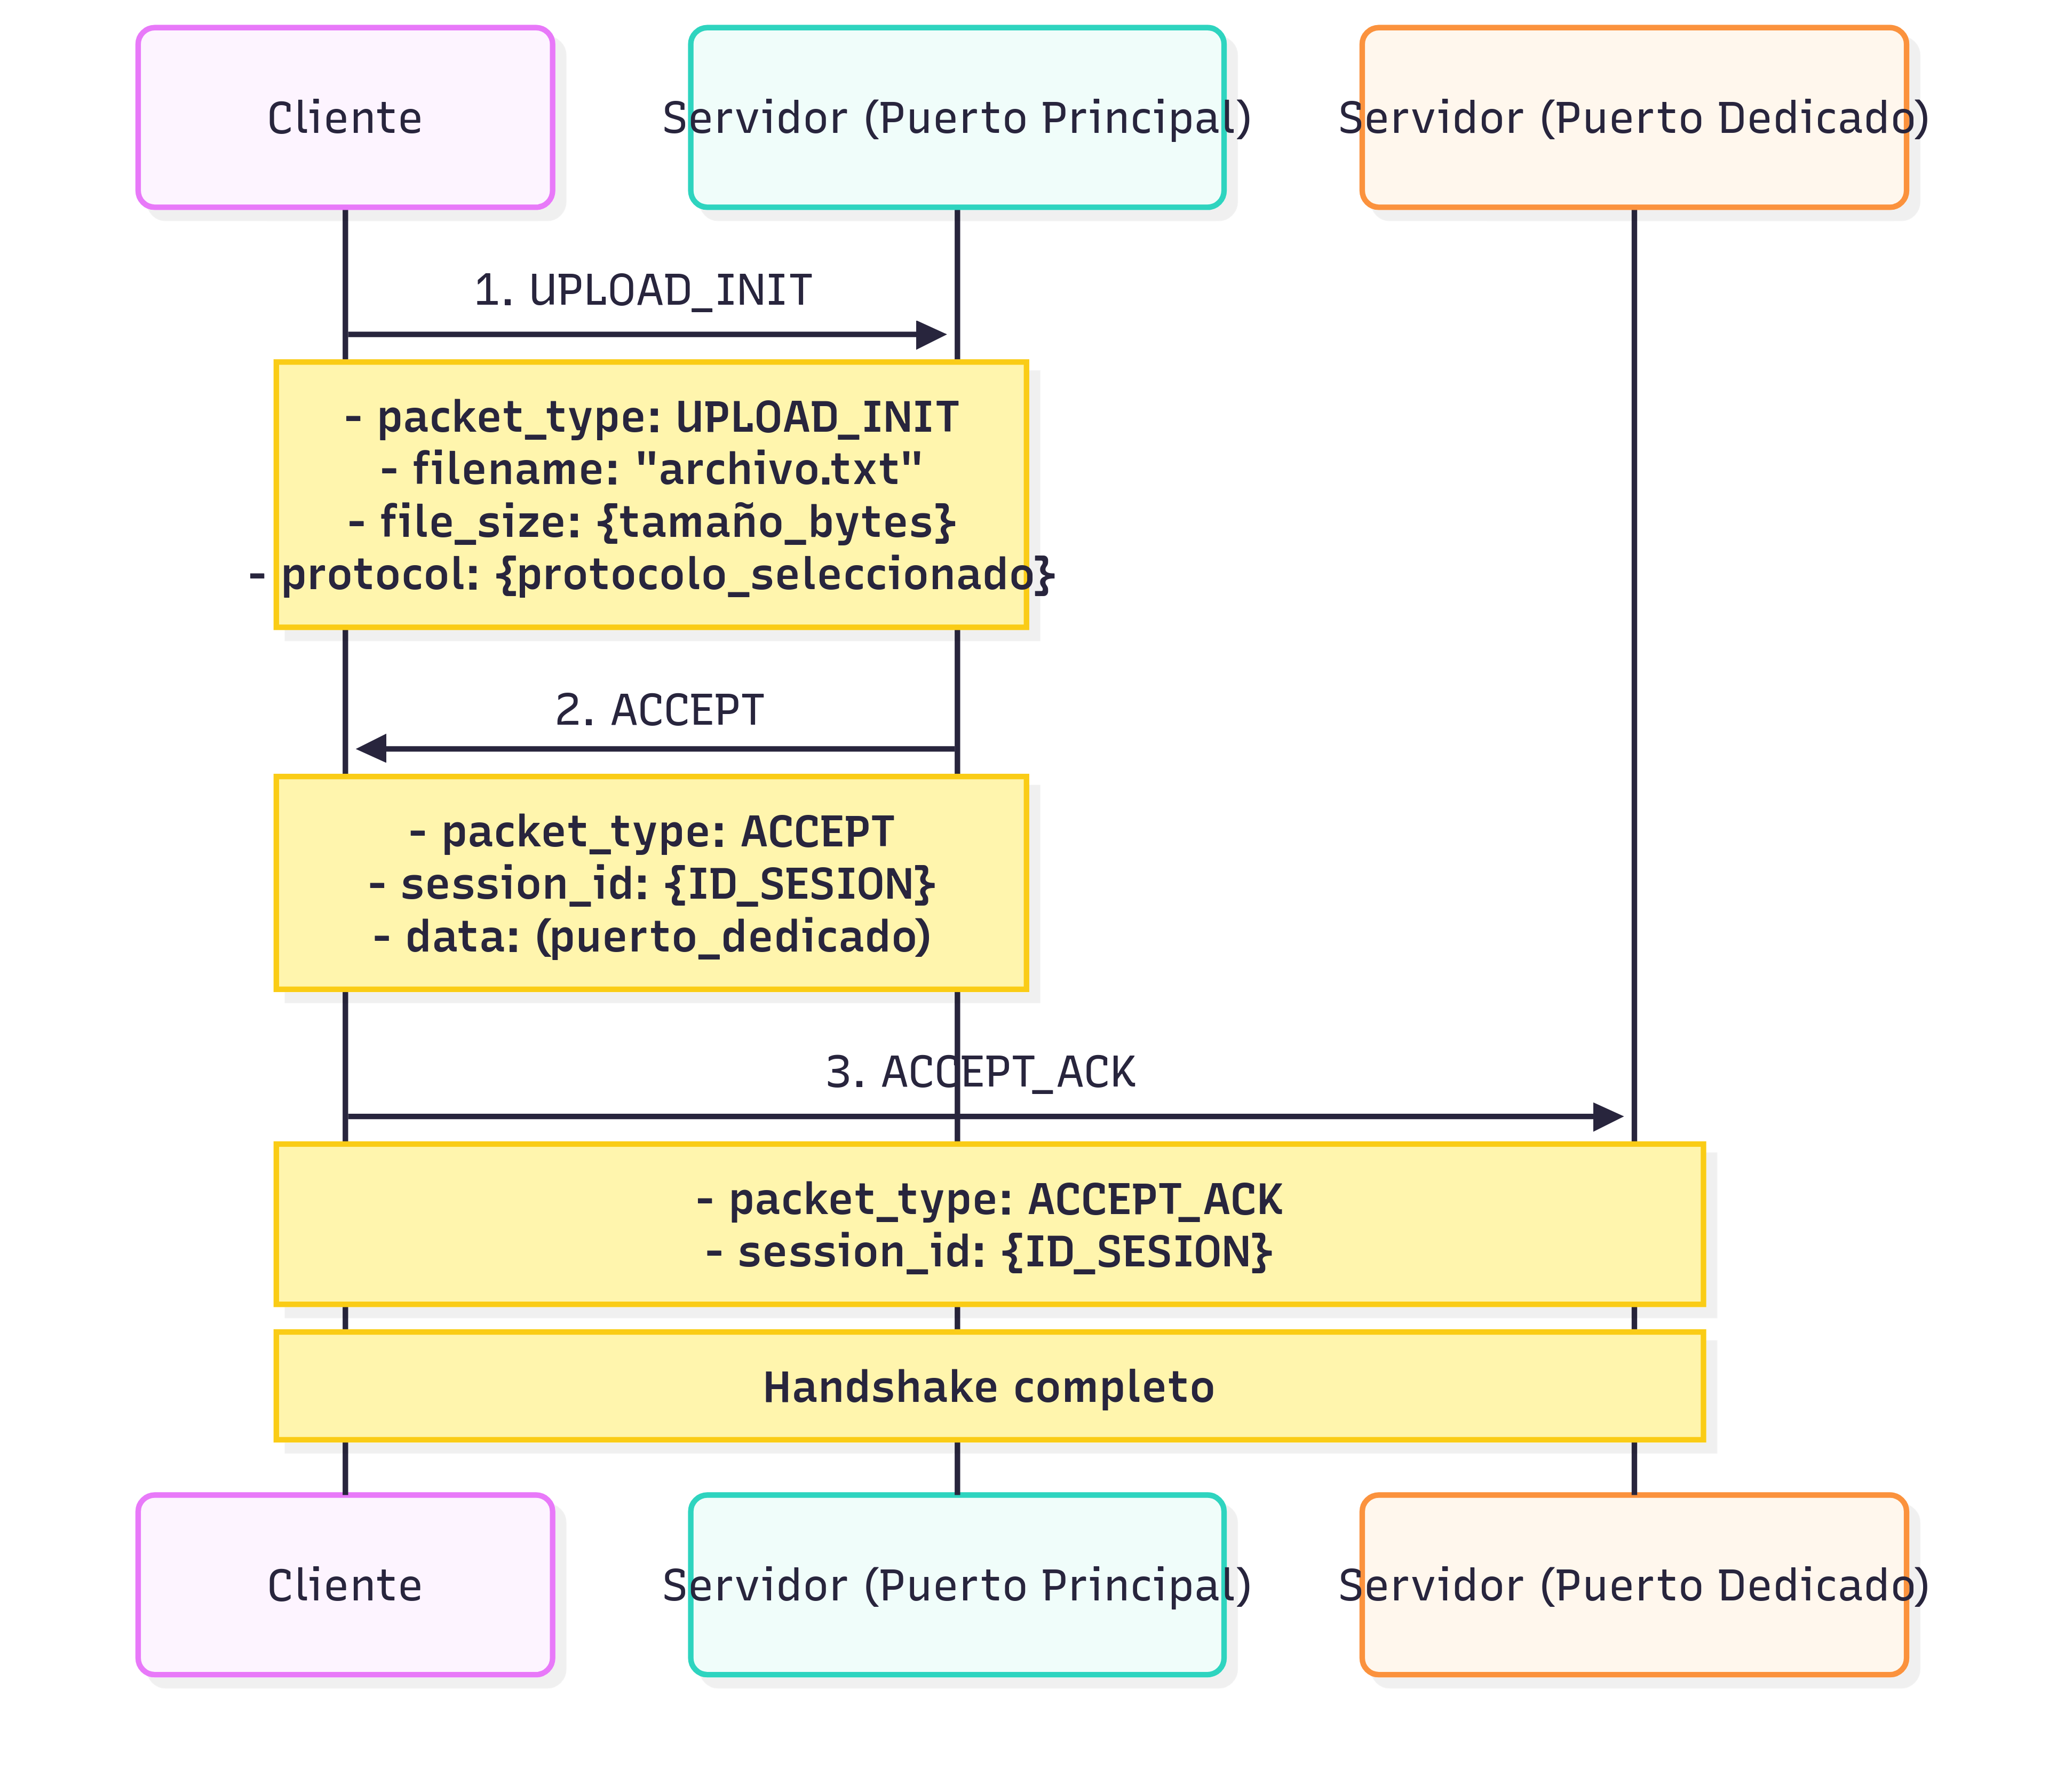
\includegraphics[width=1\linewidth]{images/UPLOAD_HANDSHAKE}
    \caption{Handshake inicial para subida de archivo}
    \label{fig:upload_handshake}
\end{figure}

\subsubsection{Handshake (download)}

\begin{figure}[H]
    \centering
    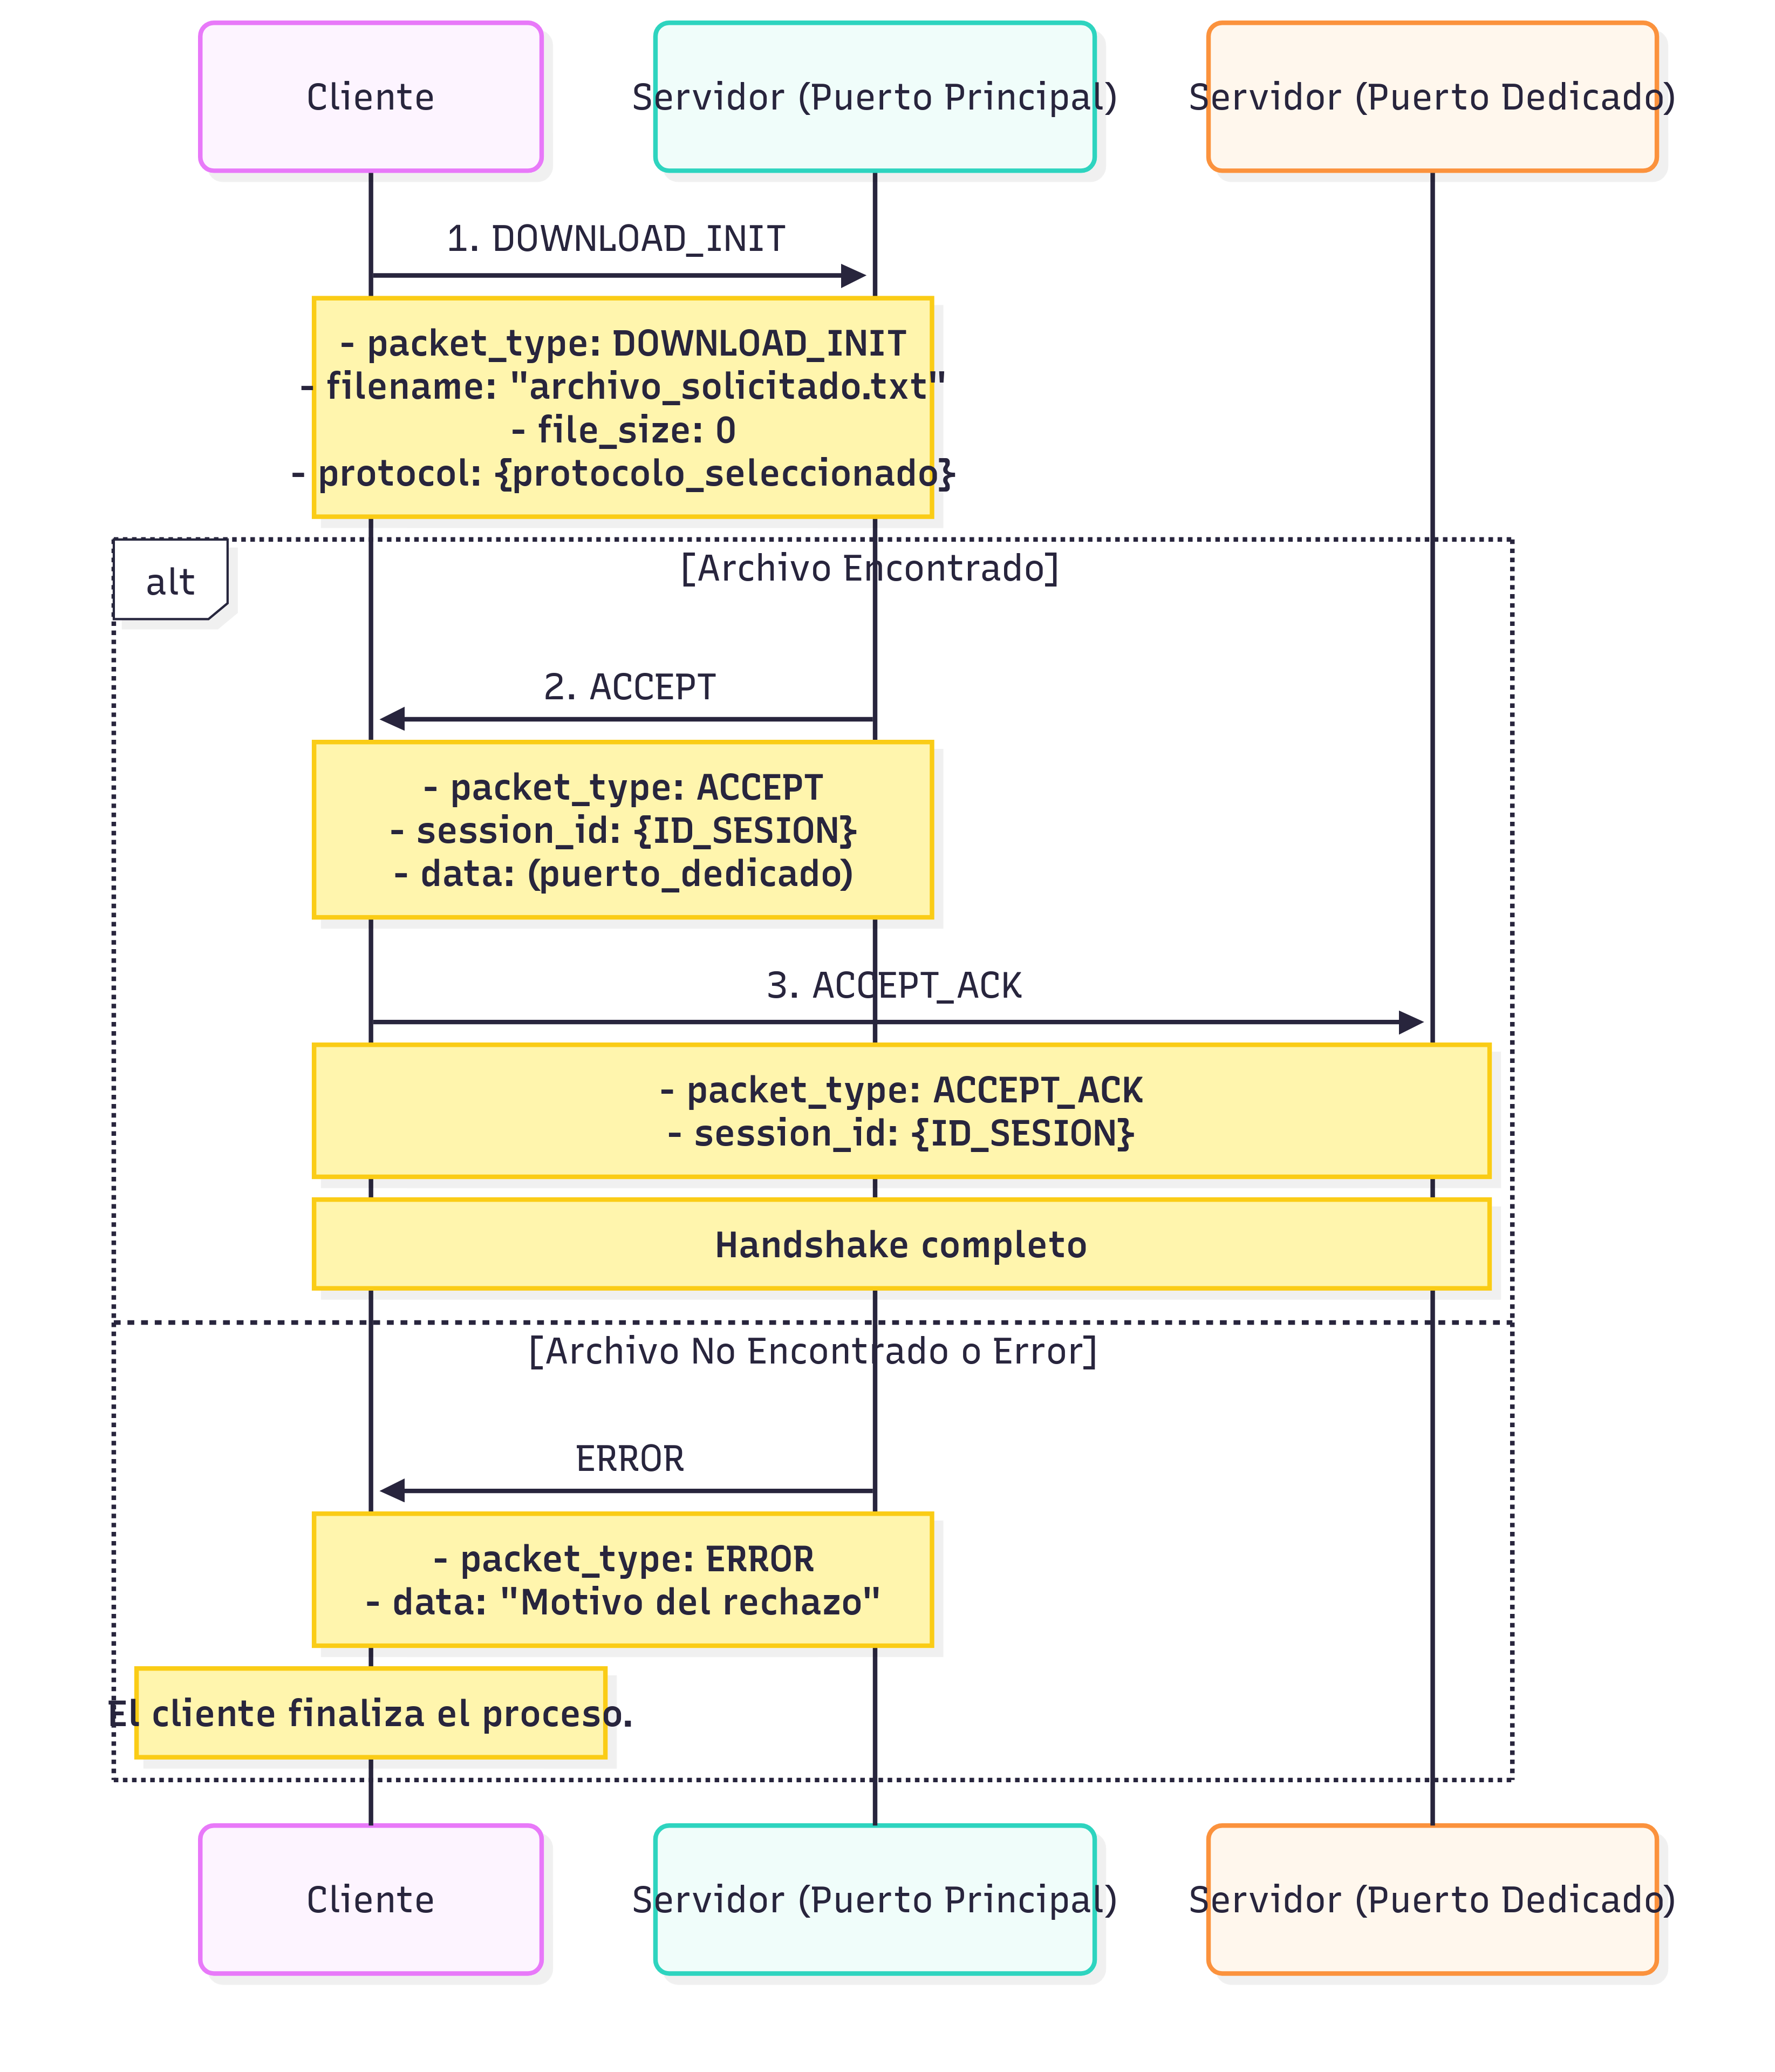
\includegraphics[width=1\linewidth]{images/DOWNLOAD_HANDSHAKE}
    \caption{Handshake inicial para descarga de archivo}
    \label{fig:download_handshake}
\end{figure}

\subsubsection{Cierre de conexion}

\begin{figure}[H]
    \centering
    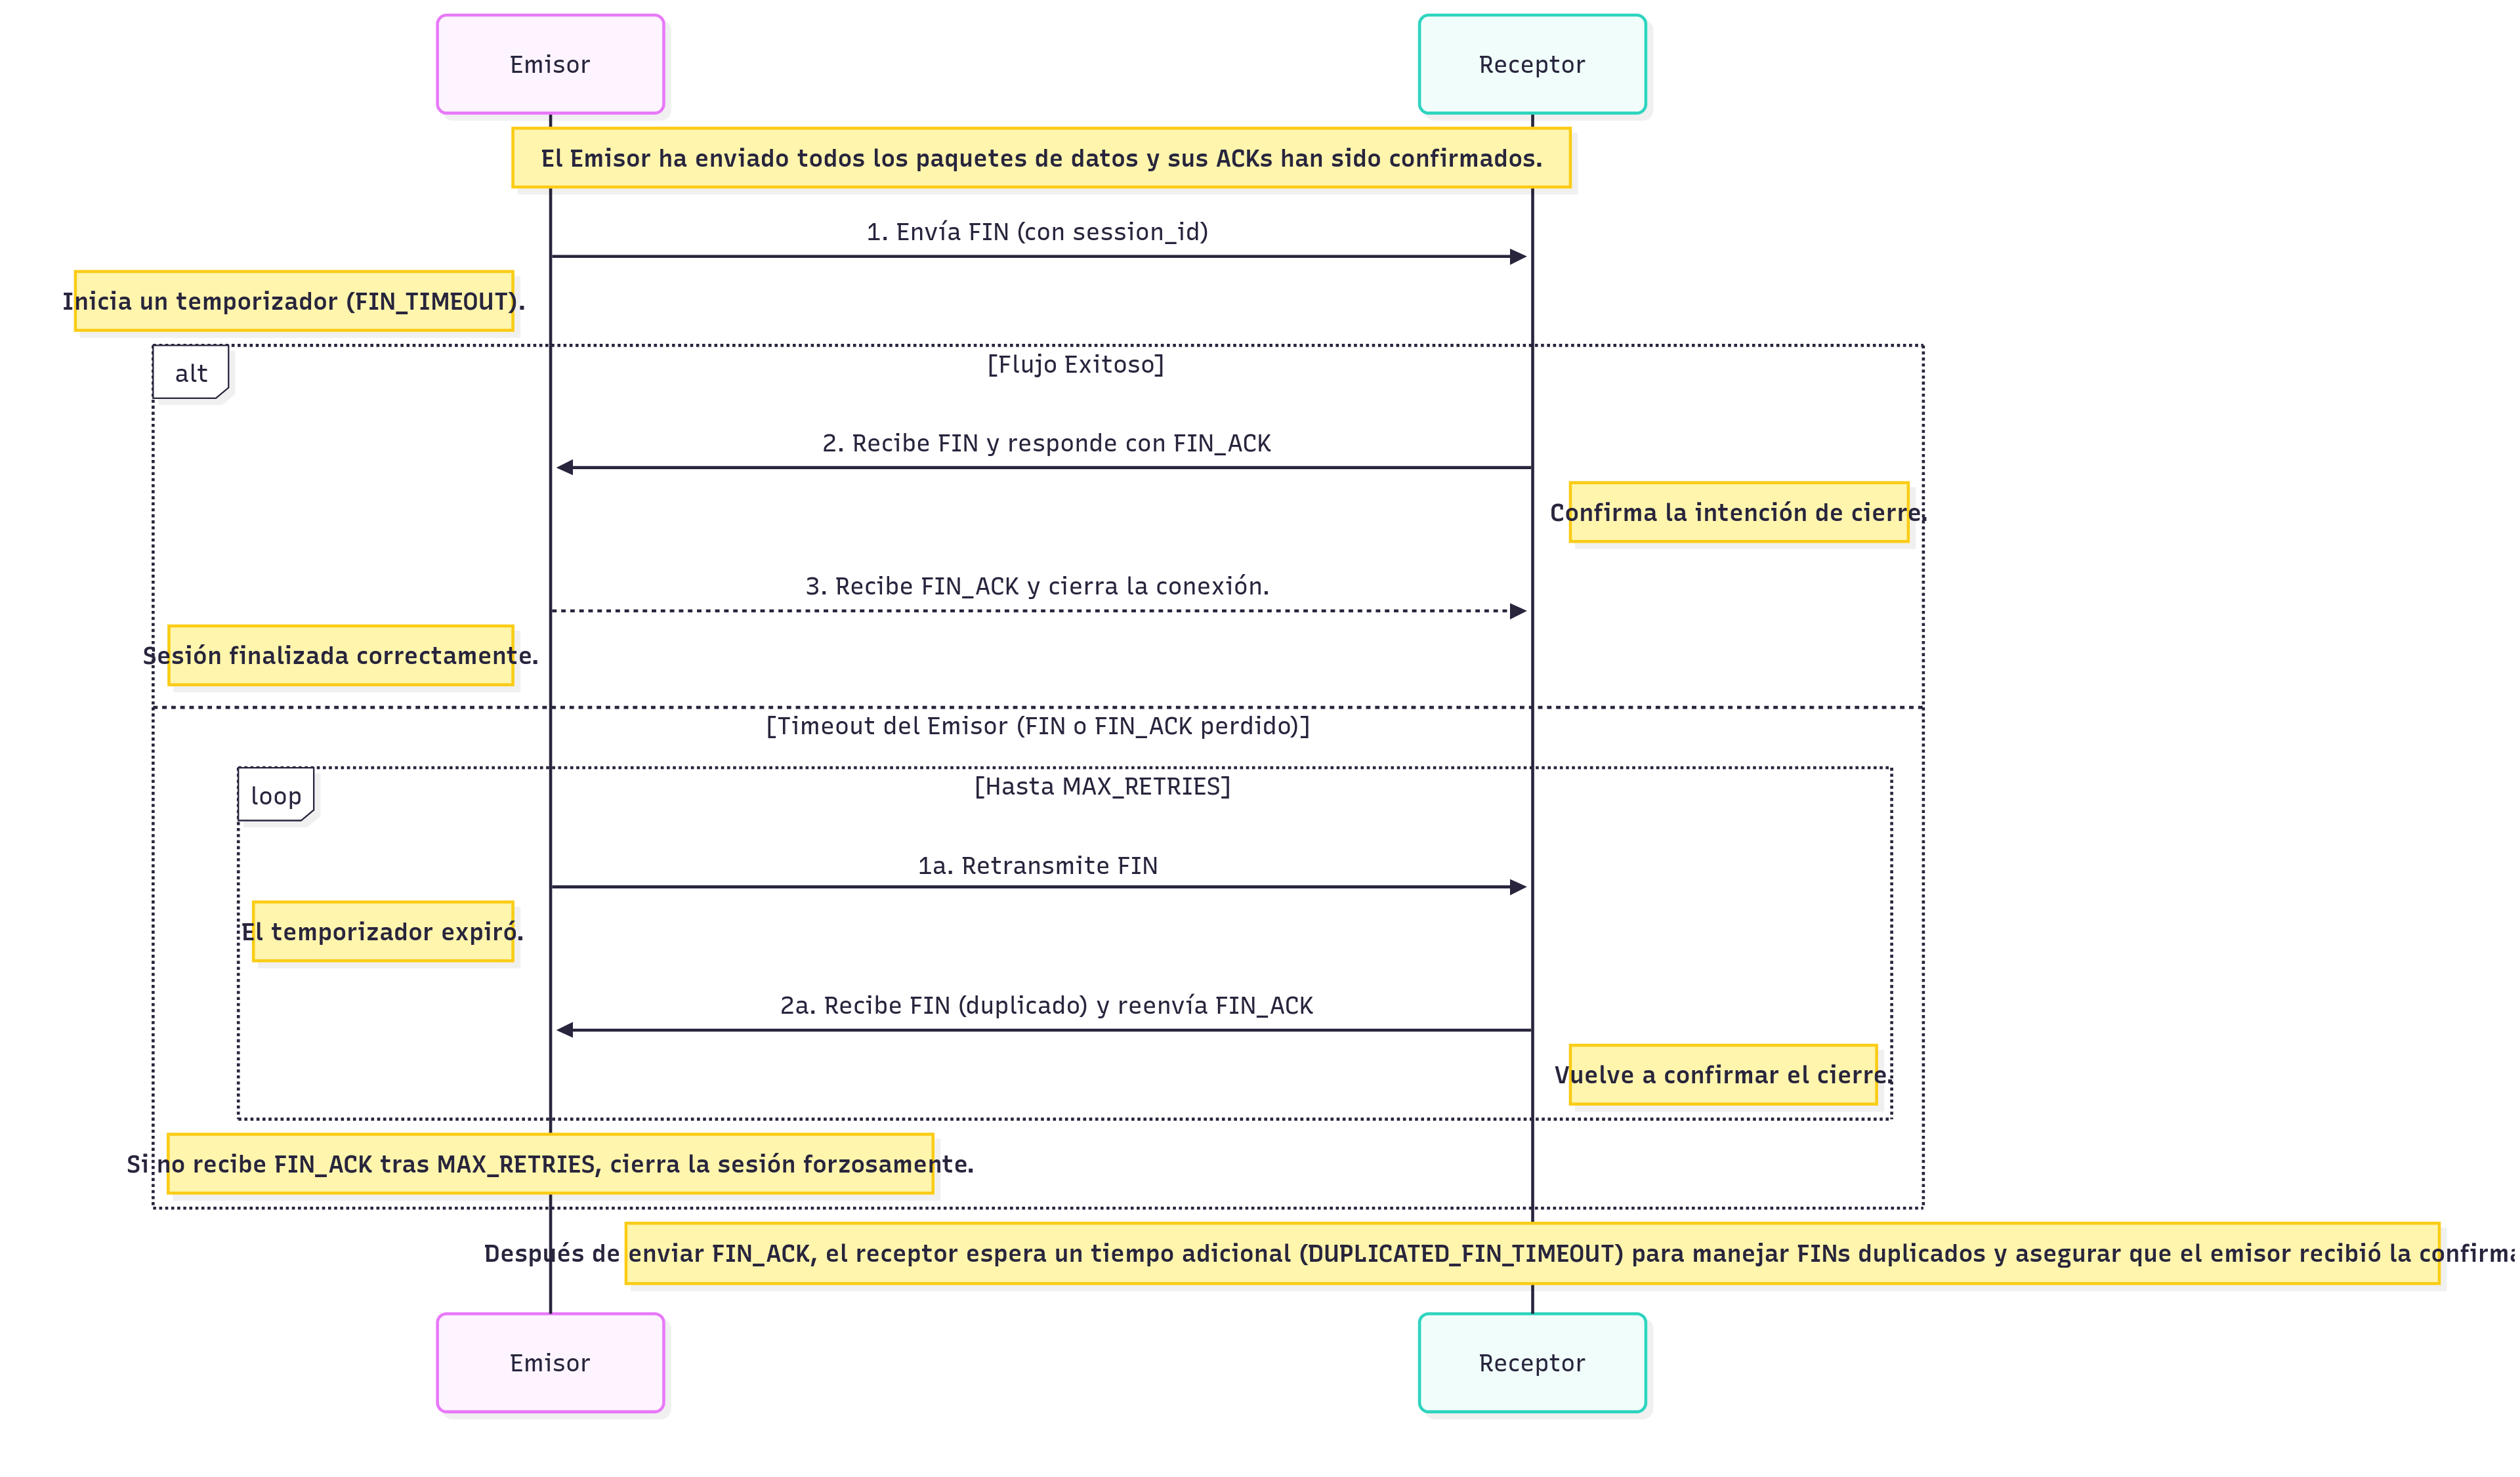
\includegraphics[width=1\linewidth]{images/FIN}
    \caption{Subida / Descarga de archivo con Selective Repeat}
    \label{fig:fin_transfer}
\end{figure}

\subsubsection{Subida / Descarga de archivo}
En el caso de una subida de archivo, el emisor es el Cliente y el receptor el Servidor. En el caso de una descarga, el emisor es el Servidor y el receptor el Cliente. El flujo de envio de paquetes DATA es el mismo para ambos casos.
\begin{figure}[H]
    \centering
    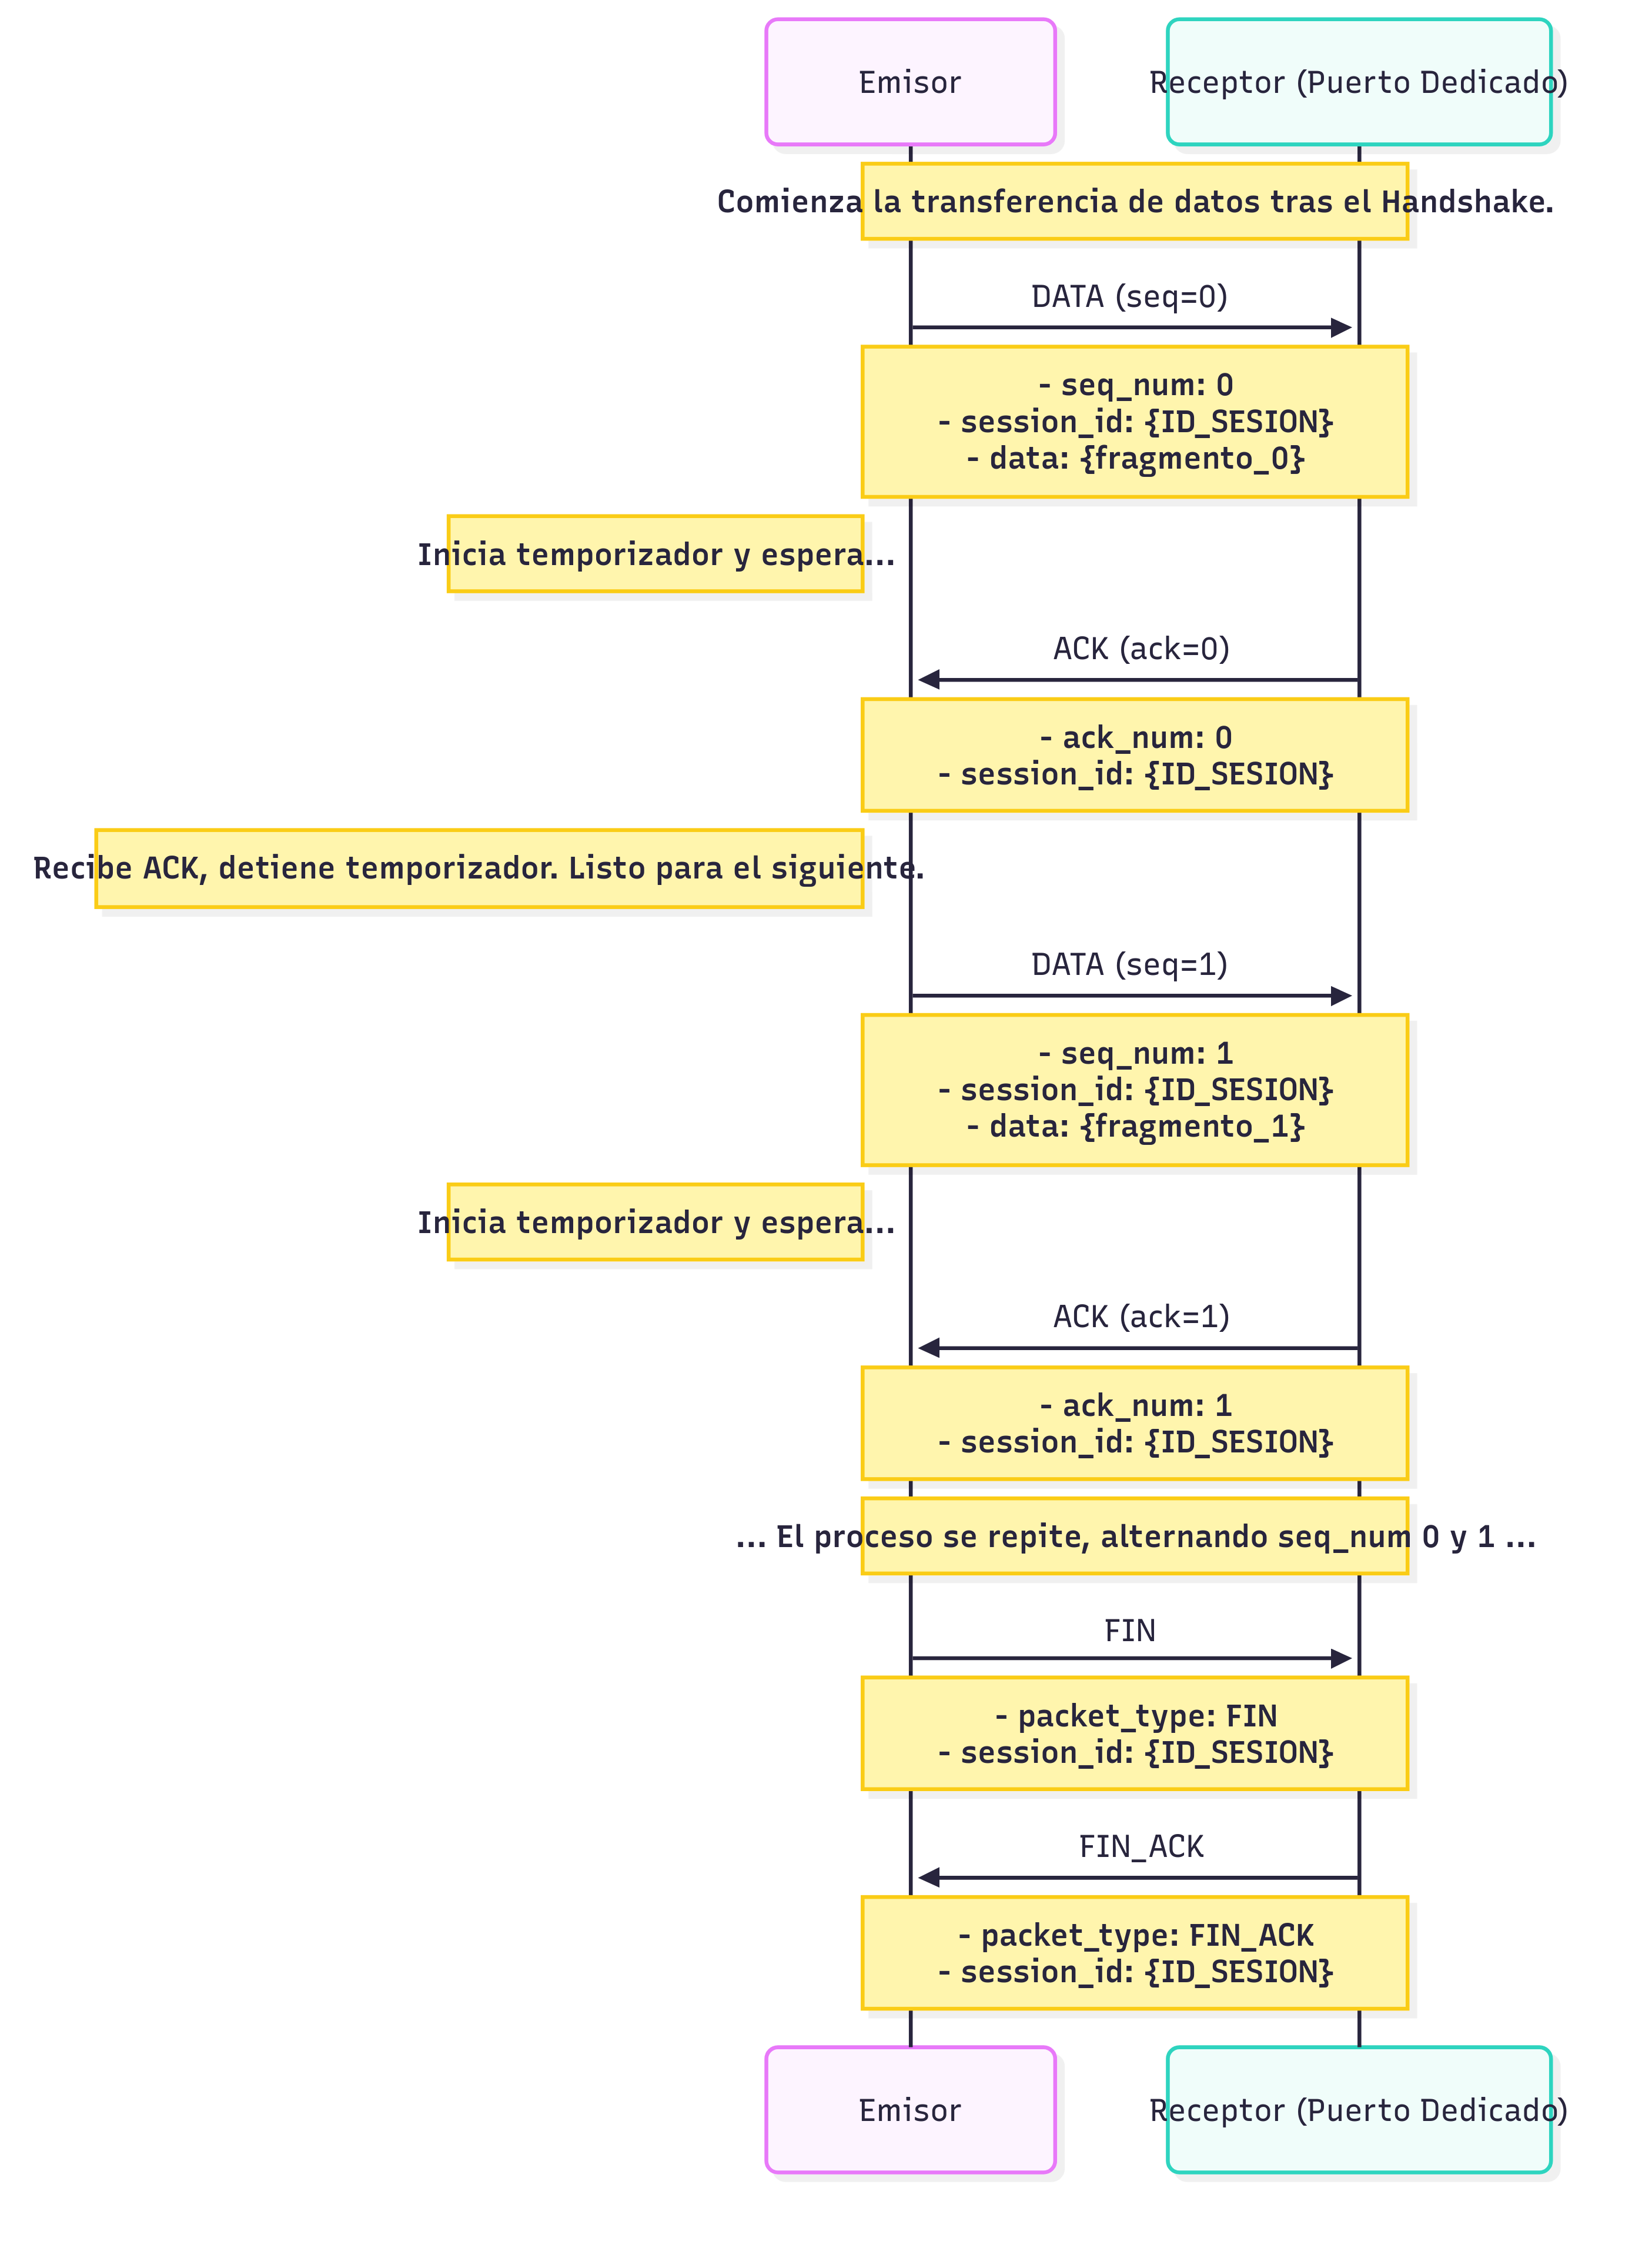
\includegraphics[height=0.8\textheight]{images/UPLOAD_DOWNLOAD}
    \caption{Subida / Descarga de archivo con Stop \& Wait}
    \label{fig:upload_download_sw}
\end{figure}

\begin{figure}[H]
    \centering
    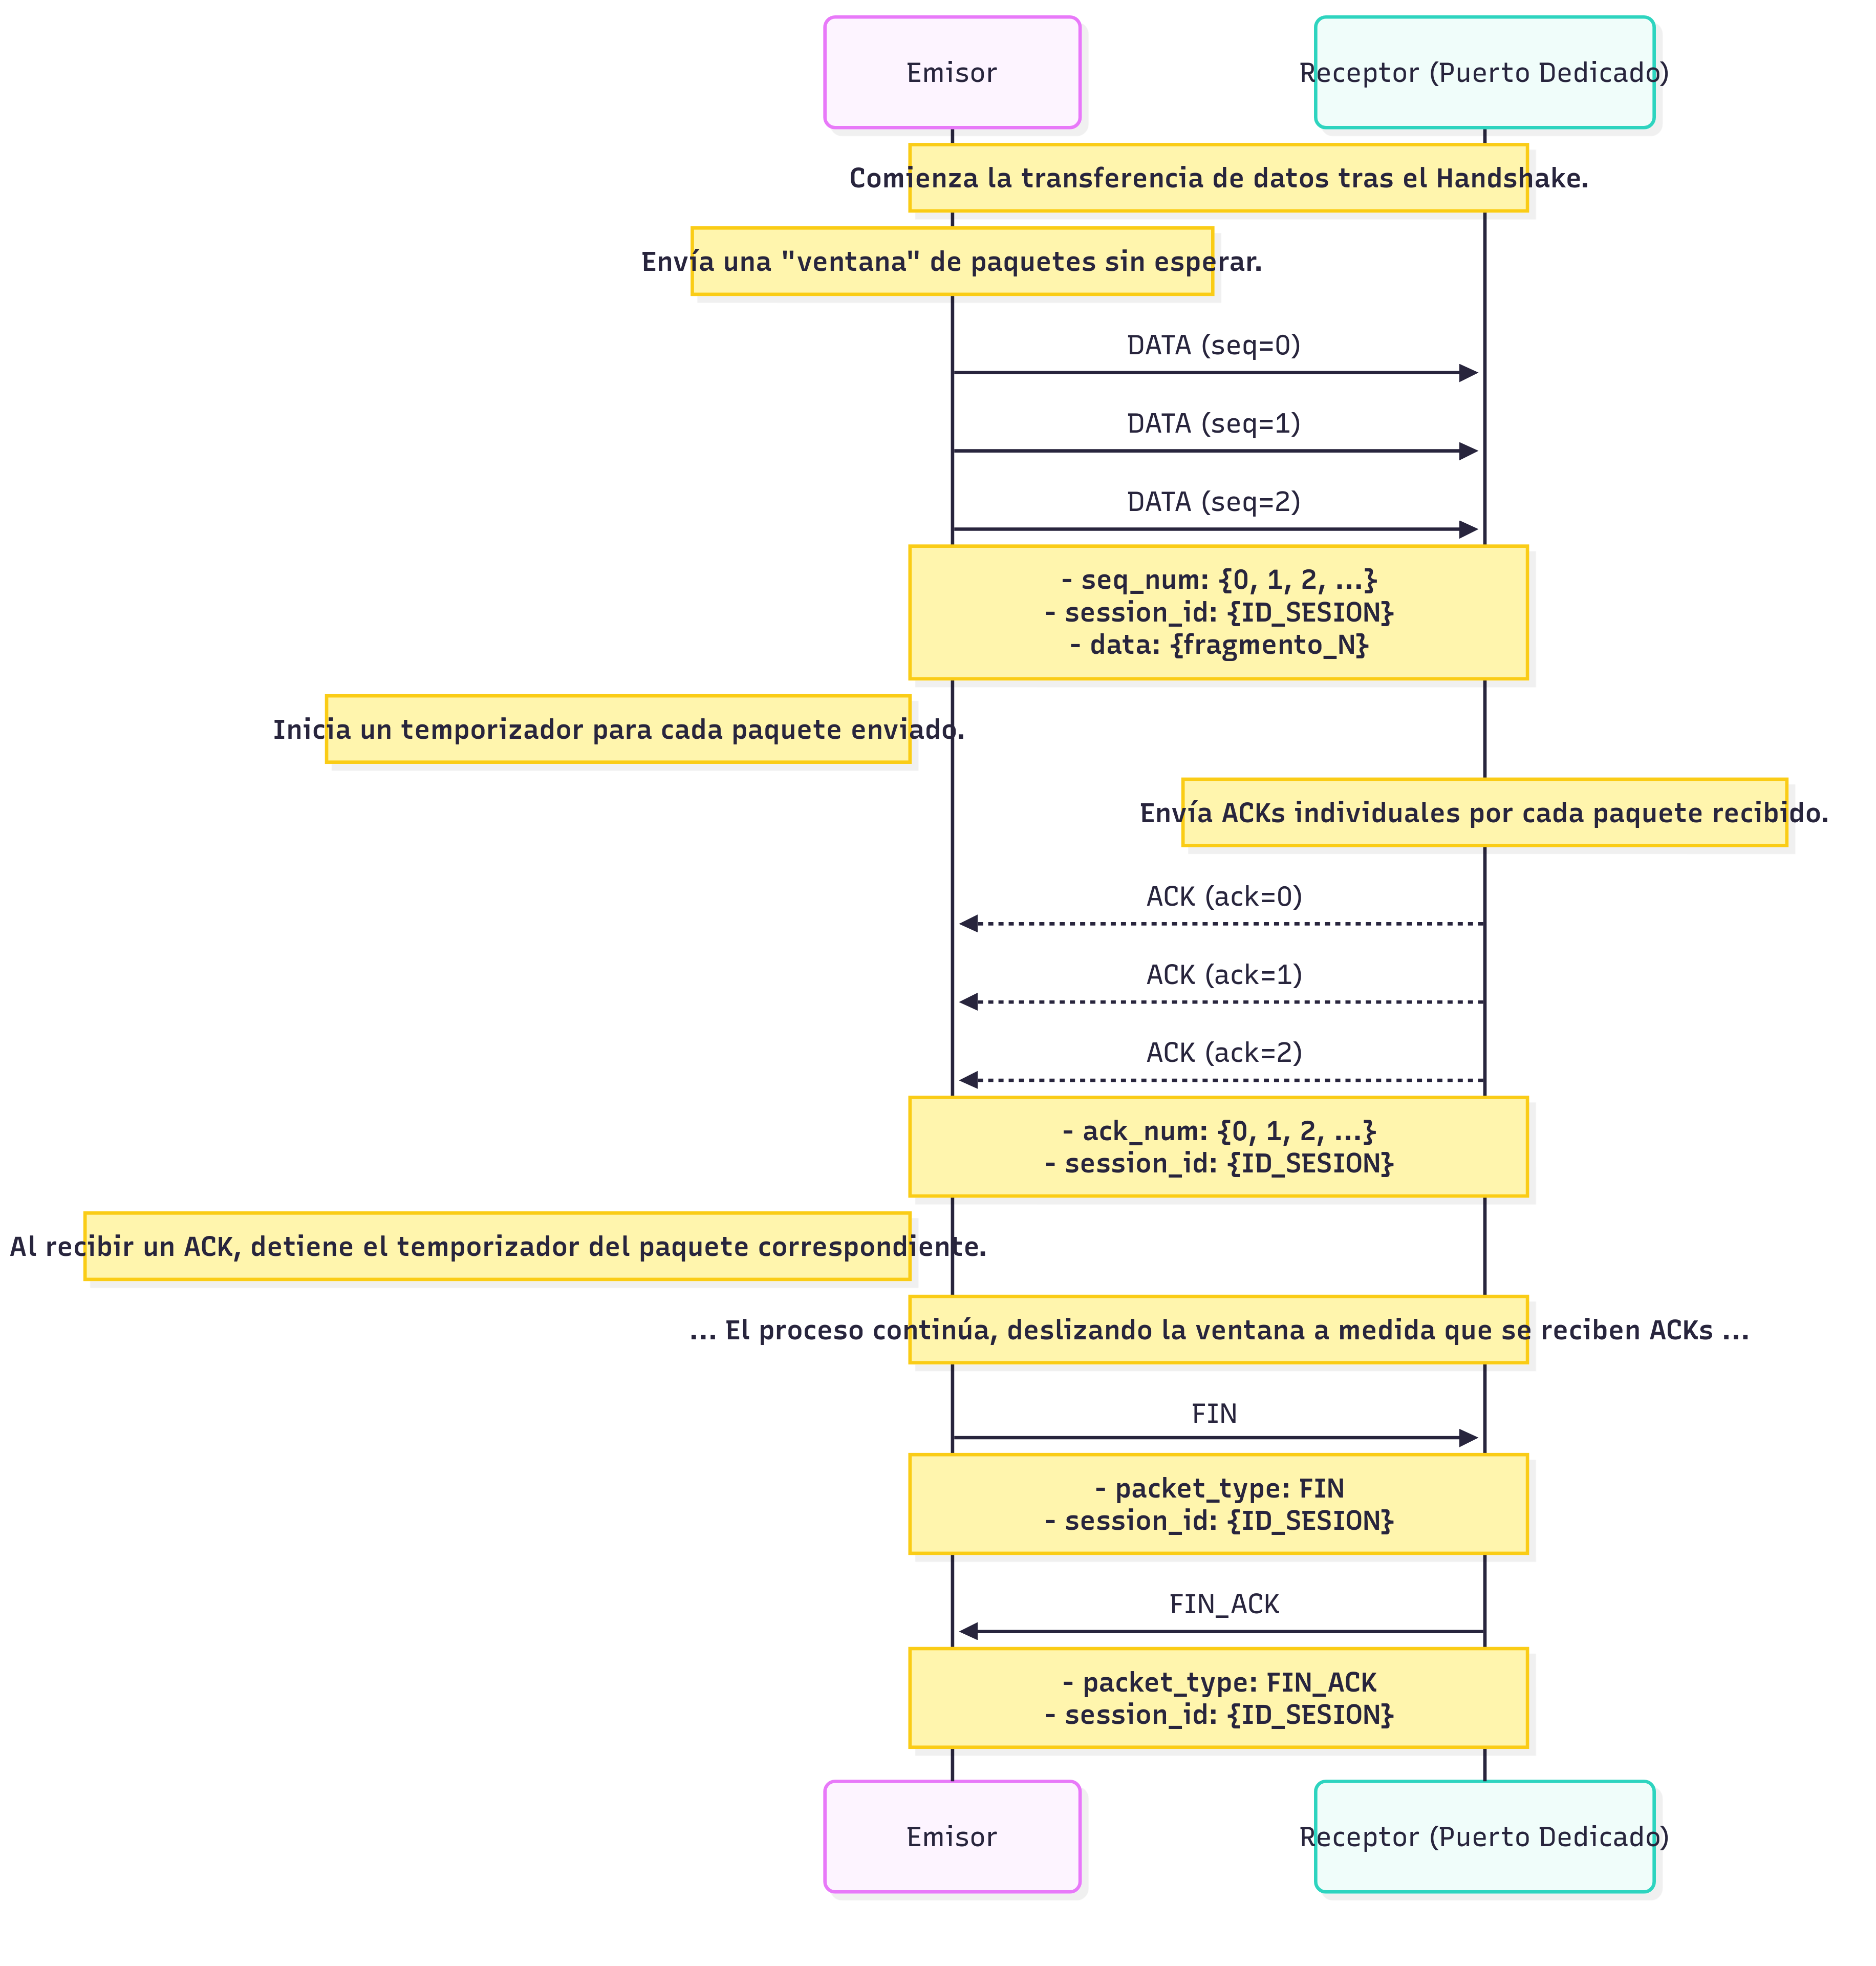
\includegraphics[height=0.8\textheight]{images/UPLOAD_DOWNLOAD_SR}
    \caption{Subida / Descarga de archivo con Selective Repeat}
    \label{fig:upload_download_sr}
\end{figure}

\subsection{Manejo de errores}
El sistema implementa múltiples capas de manejo de errores:

\begin{enumerate} [label=\roman*. , leftmargin=2cm]
    \item \textbf{Validación de Checksums:}\\
    Cada paquete incluye un checksum simple (suma de los bytes del payload, metadatos y encabezado). El receptor valida la integridad recalculando el checksum y comparándolo. En caso de que el paquete este corrupto, se descarta y no se envía confirmación, forzando retransmisión por timeout.

    \item \textbf{Timeouts y Retransmisiones:}\\
    Cada emisor asocia un temporizador a los paquetes enviados, si no se recibe el ACK correspondiente dentro del tiempo configurado, el paquete se retransmite asegurando la entrega aún bajo pérdidas del 10\% simuladas en Mininet.

    \item \textbf{Control de duplicados:}\\
    Stop \& Wait: gracias al uso de números de secuencia binarios (0/1), el receptor distingue duplicados fácilmente.\\
    Selective Repeat: mantiene una ventana deslizante con buffer y descarta paquetes ya recibidos fuera de ventana.

    \item \textbf{Manejo de paquetes fuera de orden:}\\
    Stop \& Wait: no admite desorden, cualquier paquete inesperado se ignora.\\
    Selective Repeat: almacena los paquetes válidos recibidos fuera de orden en el buffer, enviando igualmente ACKs, hasta que pueda reconstruir el flujo completo.

    \item \textbf{Mensajes de control específicos:}\\
    ERROR: permite rechazar solicitudes inválidas (por ejemplo, archivo inexistente o en uso) \\
    FIN / FIN-ACK: asegura el cierre limpio de la sesión, evitando que un corte abrupto deje la conexión en estado inconsistente.

\end{enumerate}
A continuación, se presentan diagramas de secuencia que ilustran lo explicado en algunos de los items anteriores:

\begin{figure}[H]
    \centering
    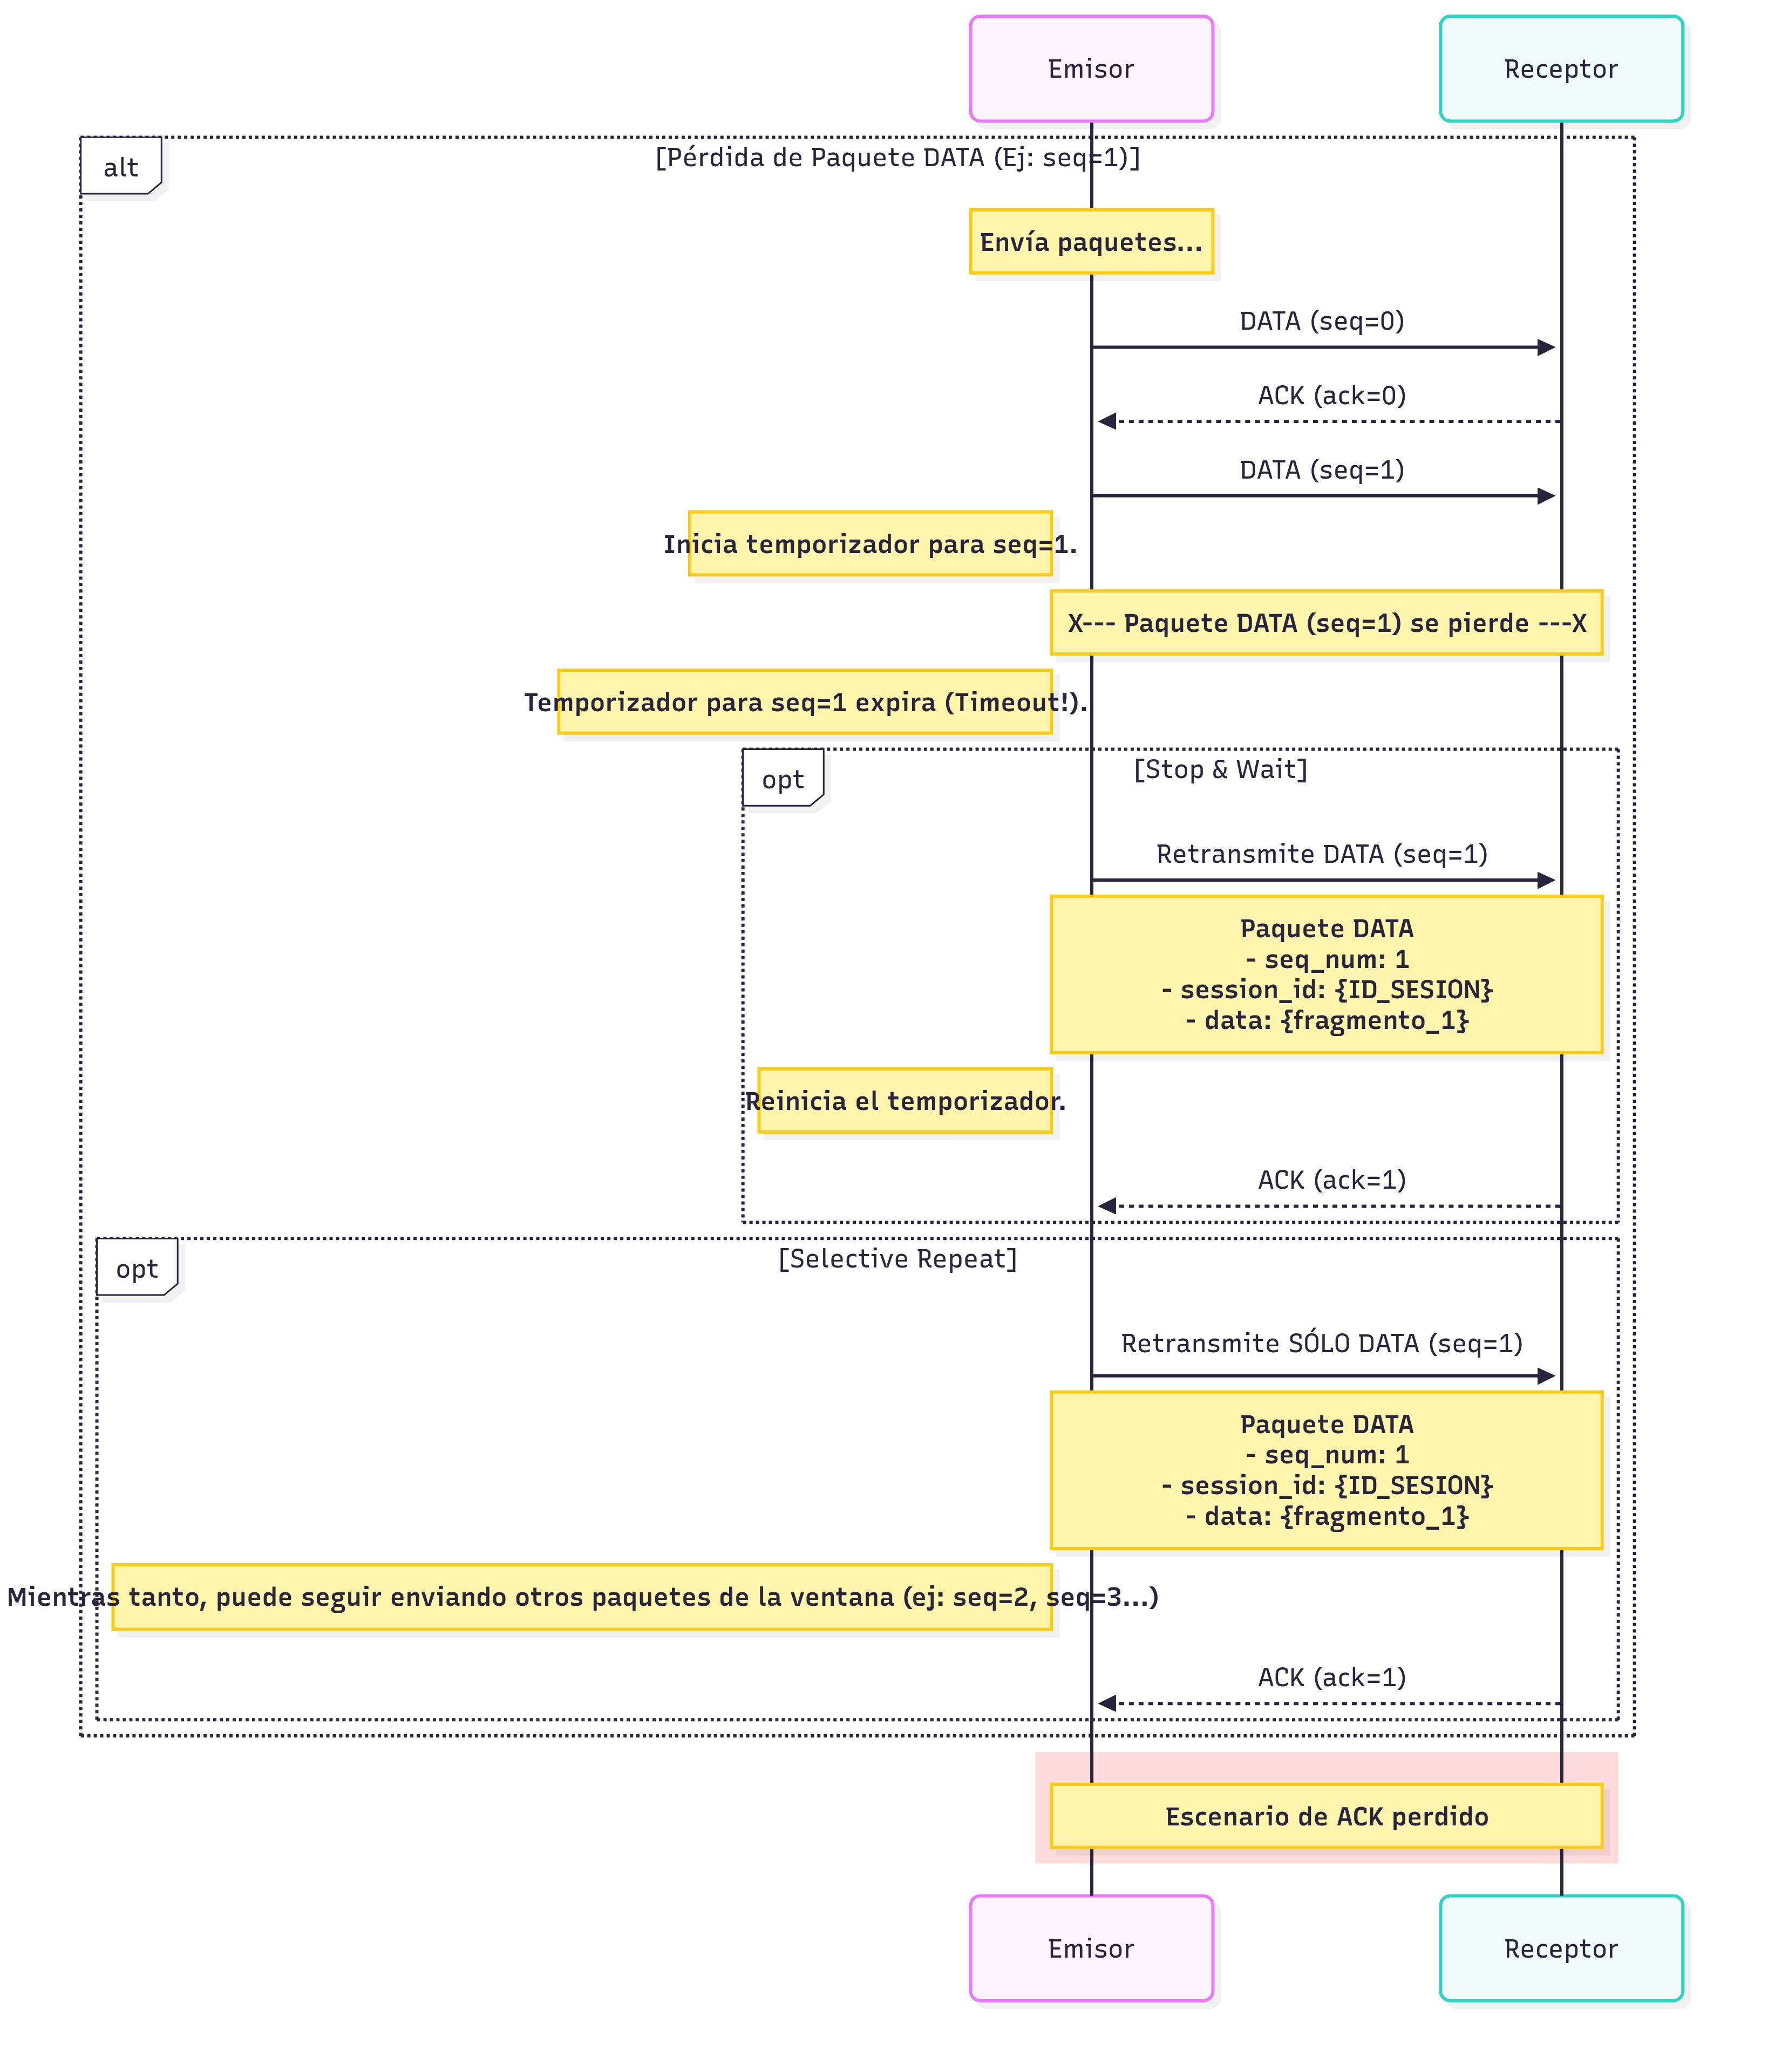
\includegraphics[width=1\linewidth]{images/RETRANSMISION}
    \caption{Retramision de paquetes por timeout.}
    \label{fig:retransmision}
\end{figure}

\begin{figure}[H]
    \centering
    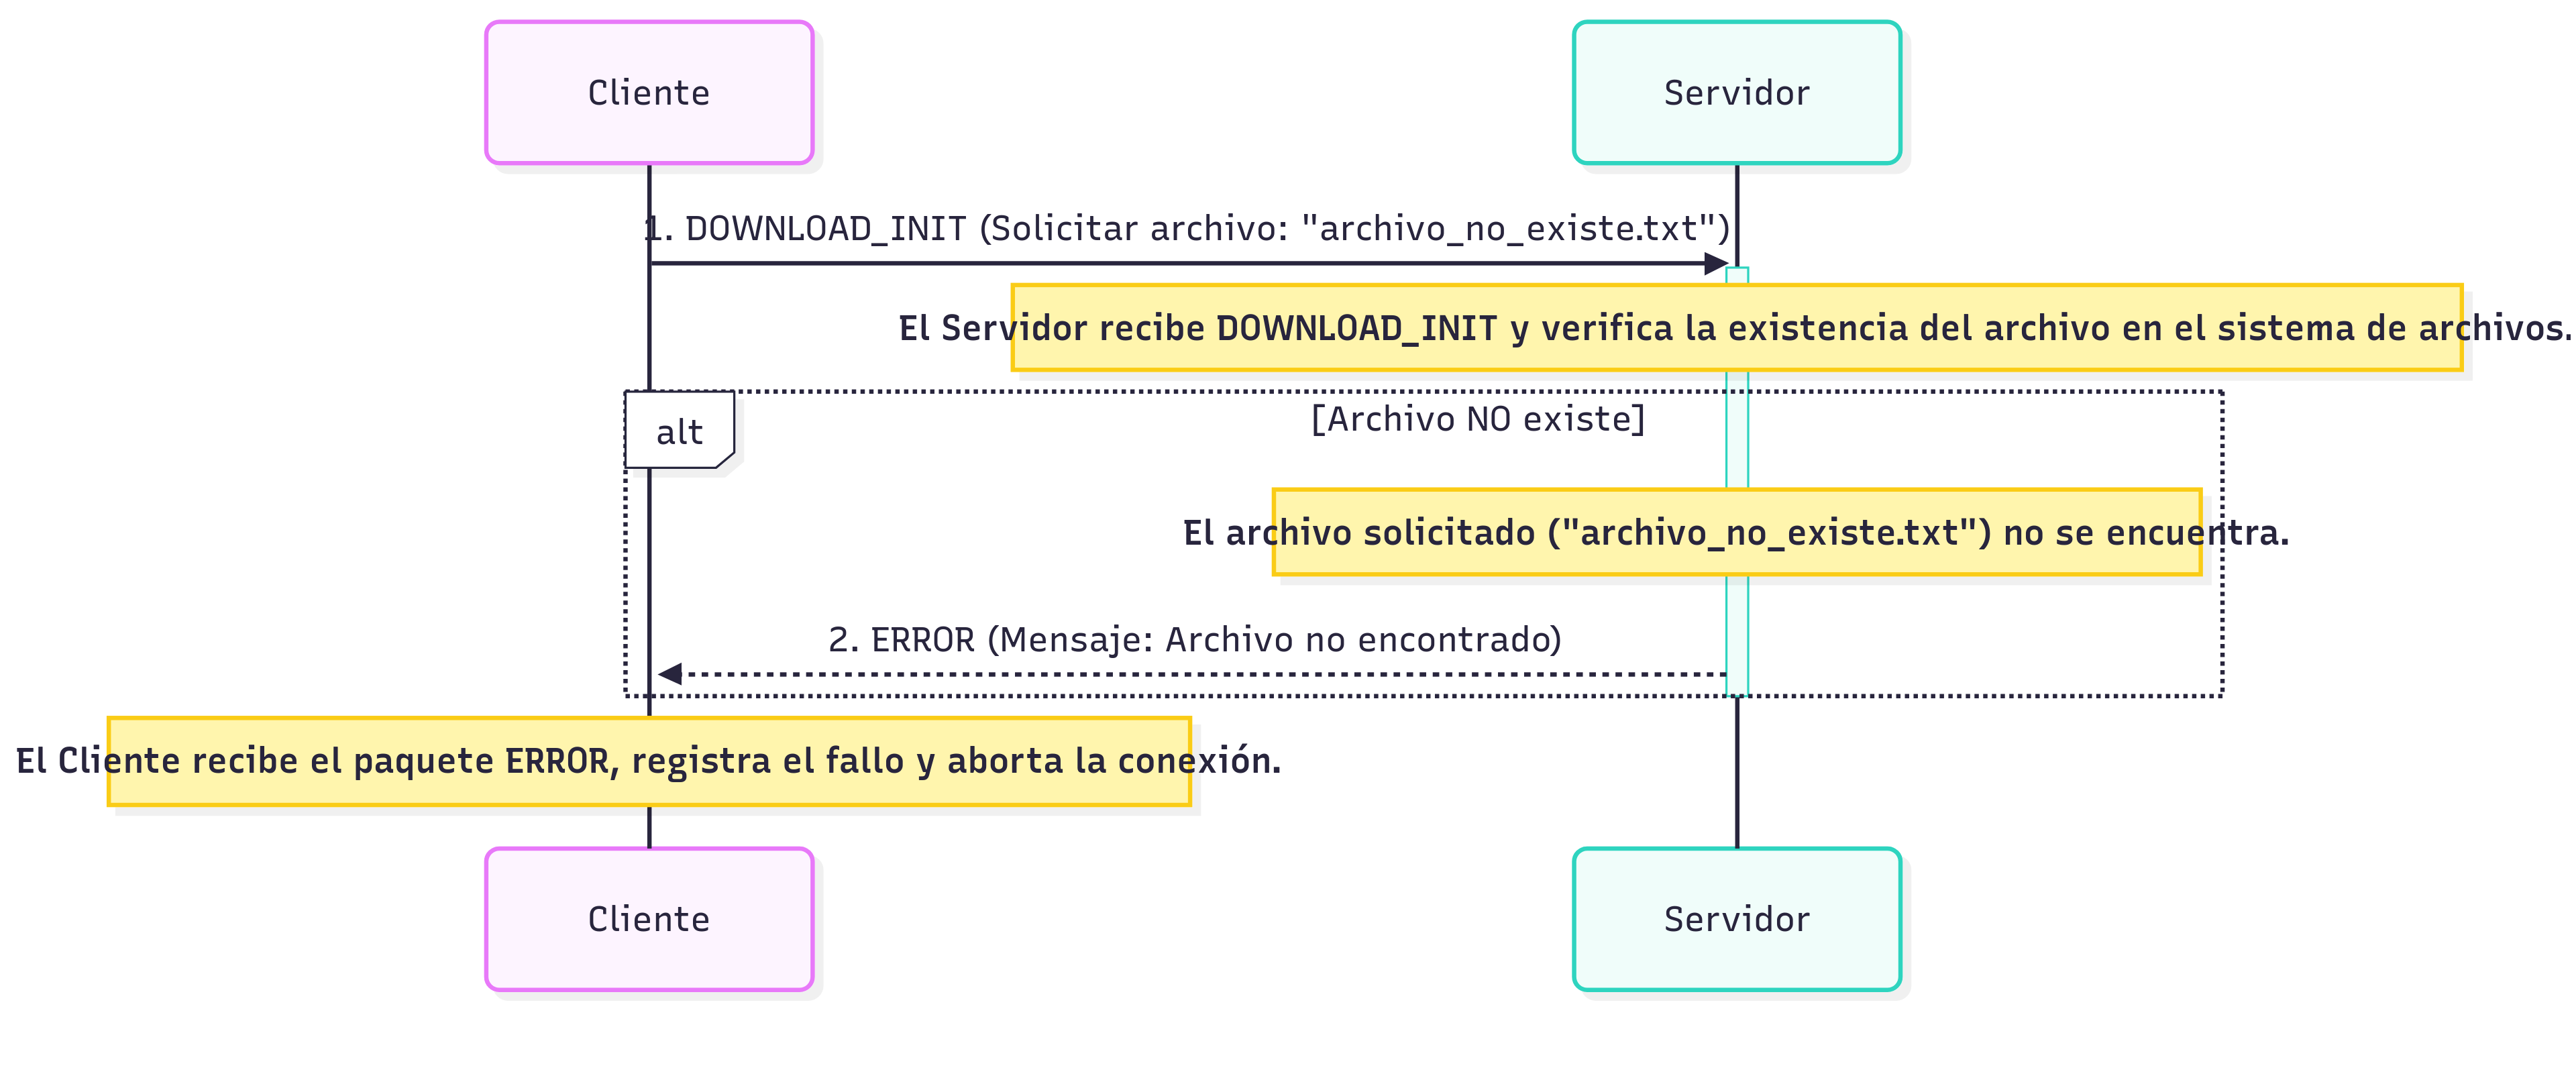
\includegraphics[width=1\linewidth]{images/diagram_sec_unexistent_file.png}
    \caption{Cierre de conexión y envio de error por solicitud de archivo inexistente.}
    \label{fig:unexistent_file_error}
\end{figure}

\subsection{Manejo de Concurrencia}

\subsubsection{Arquitectura Concurrente}
El servidor implementado es capaz de atender múltiples clientes simultáneamente sin que las transferencias interfieran entre sí.
El servidor utiliza un modelo de concurrencia basado en threads con recursos dedicados por sesión. La arquitectura se puede describir en tres niveles:
\\

\textbf{Thread Principal (Main Thread)}

El thread principal del servidor ejecuta un loop infinito que:

\begin{enumerate}
    \item Escucha en el puerto principal (49153) solicitudes de inicio de transferencia
    \item Valida que haya capacidad disponible
    \item Crea recursos dedicados para cada nueva transferencia
    \item Delega el manejo de la transferencia a un thread dedicado
    \item Registra la sesión en el diccionario de sesiones activas
\end{enumerate}

Este diseño permite que el thread principal continúe aceptando nuevas conexiones mientras las transferencias en curso se ejecutan en paralelo.
\\

\textbf{Threads Dedicados (Worker Threads)}

Cada transferencia corre en su propio thread con recursos completamente aislados:

\begin{itemize}
    \item \textbf{Socket UDP dedicado:} Cada sesión tiene su propio socket escuchando en un puerto dinámico único
    \item \textbf{Session ID único:} Identificador de 1-255 que no colisiona con otras sesiones activas
    \item \textbf{Estado independiente:} Variables de protocolo (ventanas, buffers) no compartidas entre threads
    \item \textbf{File descriptor:} Cada thread maneja su propio archivo sin compartir recursos de I/O
\end{itemize}

Este aislamiento garantiza que un error o problema en una transferencia no afecta a las demás.

\subsubsection{Gestión de Recursos Compartidos}

Aunque cada transferencia está mayormente aislada, existen algunos recursos compartidos que requieren sincronización cuidadosa:
\\

\textbf{Diccionario de Sesiones Activas}

El servidor mantiene un diccionario global de todas las sesiones activas, que contiene para cada sesión:

\begin{itemize}
    \item \texttt{session\_id}: Identificador único (1-255)
    \item \texttt{dedicated\_port}: Puerto UDP asignado
    \item \texttt{thread}: Referencia al thread worker
    \item \texttt{dedicated\_socket}: Socket UDP dedicado
    \item \texttt{client\_addr}: Dirección IP y puerto del cliente
    \item \texttt{created\_at}: Timestamp de creación
\end{itemize}

Para garantizar consistencia, todas las operaciones sobre este diccionario están protegidas por un lock (\texttt{sessions\_lock}). Las operaciones sincronizadas incluyen:

\begin{itemize}
    \item Agregar nueva sesión
    \item Remover sesión completada
    \item Verificar cantidad de sesiones activas
    \item Generar session ID único
\end{itemize}

\subsubsection{Puertos Dedicados}

Cada transferencia obtiene su propio puerto UDP, lo que proporciona aislamiento a nivel de socket del sistema operativo.

\textbf{Asignación Dinámica de Puertos}

El servidor crea un socket UDP y lo vincula al puerto 0, lo que indica al sistema operativo que asigne automáticamente un puerto disponible del rango de puertos dinámicos (típicamente 49152-65535). Este mecanismo tiene varias ventajas:

\begin{enumerate}
    \item \textbf{Aislamiento completo:} Los paquetes de diferentes transferencias nunca se mezclan, ya que cada una tiene su propio socket

    \item \textbf{Sin multiplexación:} No hay necesidad de demultiplexar paquetes por session\_id en el socket principal, simplificando la lógica

    \item \textbf{Simplicidad:} Cada thread puede ejecutar \texttt{recvfrom()} sin condiciones de carrera ni coordinación con otros threads

    \item \textbf{Escalabilidad:} El sistema operativo maneja eficientemente la distribución de puertos y el enrutamiento de paquetes

    \item \textbf{Robustez:} Si un socket falla o se bloquea, no afecta a los demás
\end{enumerate}

\subsubsection{Control de Capacidad}

El servidor implementa un límite configurable de transferencias concurrentes para prevenir agotamiento de recursos del sistema.

Antes de aceptar una nueva transferencia, el servidor verifica que el número de sesiones activas no supere el máximo configurado (10 por defecto). Si el servidor está a capacidad:

\begin{enumerate}
    \item Se registra una advertencia en los logs
    \item Se envía un paquete ERROR al cliente con el mensaje ``Server at capacity, try again later''
    \item Se rechaza la conexión sin crear recursos
    \item El cliente puede reintentar más tarde
\end{enumerate}

\subsubsection{Flujo Completo de una Sesión Concurrente}

A continuación se describe el ciclo de vida completo de una sesión en el servidor concurrente:

\begin{figure}[H]
\centering
\small
\begin{minipage}{0.9\textwidth}
\begin{verbatim}
1. Cliente envia UPLOAD_INIT/DOWNLOAD_INIT al puerto 49153
   |
   +---> Thread Principal recibe solicitud
   |    |
   |    +---> Adquiere lock sobre sessions_lock
   |    +---> Verifica capacidad (< 10 sesiones)
   |    +---> Libera lock
   |
   +---> Si capacidad disponible:
   |    |
   |    +---> Genera session_id unico (con lock)
   |    +---> Crea socket dedicado en puerto N
   |    +---> Envia ACCEPT(session_id, puerto N)
   |    |
   |    +---> Crea thread dedicado T
   |    +---> Registra sesion en active_sessions (con lock)
   |    +---> Inicia thread: T.start()
   |
   +---> Si capacidad completa:
        +---> Envia ERROR("Server at capacity")

2. Thread Dedicado T ejecuta:
   |
   +---> Espera ACCEPT_ACK en socket dedicado
   +---> Crea instancia de protocolo (Stop&Wait o Selective Repeat)
   +---> Ejecuta transferencia (bloqueante solo para este thread)
   +---> Guarda archivo en disco
   |
   +---> Finally (siempre ejecuta):
        +---> Adquiere lock sobre sessions_lock
        +---> Elimina sesion de active_sessions
        +---> Libera lock
        +---> Cierra socket dedicado

3. Thread Principal continua:
   +---> Loop: Espera proxima solicitud (no bloqueado por T)
\end{verbatim}
\end{minipage}
\caption{Ciclo de vida de una sesión concurrente}
\end{figure}

\subsection{Stop \& Wait}

Stop \& Wait es el protocolo RDT más simple implementado en este trabajo. Su funcionamiento se basa en el envío secuencial de paquetes: el emisor transmite un paquete y espera la confirmación (ACK) antes de enviar el siguiente.

\subsubsection{Principio de funcionamiento}

El protocolo utiliza números de secuencia alternantes (0 y 1) para distinguir entre paquetes consecutivos y detectar duplicados. El emisor mantiene una variable \texttt{seq\_num} que alterna entre 0 y 1 con cada paquete enviado exitosamente, mientras que el receptor mantiene una variable \texttt{expected\_seq} que indica el número de secuencia del próximo paquete esperado.

El flujo básico es:
\begin{enumerate}
    \item Emisor envía paquete con \texttt{seq\_num = n}
    \item Emisor inicia timer y espera ACK
    \item Receptor recibe paquete, verifica checksum y número de secuencia
    \item Si el paquete es correcto y tiene el \texttt{seq\_num} esperado:
    \begin{itemize}
        \item Receptor acepta los datos
        \item Receptor envía ACK con \texttt{ack\_num = n}
        \item Receptor incrementa \texttt{expected\_seq}
    \end{itemize}
    \item Si el paquete es duplicado o corrupto:
    \begin{itemize}
        \item Receptor descarta los datos
        \item Receptor envía ACK del paquete anterior (ACK duplicado)
    \end{itemize}
    \item Emisor recibe ACK y avanza al siguiente paquete
    \item Si timer expira antes de recibir ACK, el emisor retransmite
\end{enumerate}

\subsubsection{Implementación del emisor}

La clase \texttt{RDTSender} en \texttt{stop\_wait.py} implementa el emisor del protocolo Stop \& Wait. Sus componentes principales son:
\\

\textbf{Variables de estado:}
\begin{itemize}
    \item \texttt{seq\_num}: Número de secuencia actual (0 o 1)
    \item \texttt{session\_id}: Identificador de sesión asignado por el servidor
    \item \texttt{socket}: Socket UDP para transmisión
    \item \texttt{dest\_addr}: Dirección y puerto del receptor
\end{itemize}

 
\textbf{Preparación de paquetes:}

El método \texttt{\_prepare\_packets()} lee el archivo fuente y lo fragmenta en paquetes DATA.
\\

\textbf{Envío confiable de paquetes:}

El método \texttt{\_send\_packet\_reliable()} implementa el núcleo del protocolo. Para cada paquete:

\begin{enumerate}
    \item Se envía el paquete al receptor mediante \texttt{socket.sendto()}
    \item Se inicia un timer implícito configurando \texttt{socket.settimeout(SW\_TIMEOUT)} con un timeout de 50ms
    \item Se bloquea esperando el ACK con \texttt{socket.recvfrom()}
    \item Si se recibe un ACK válido (tipo ACK, \texttt{ack\_num} correcto, checksum válido), se retorna éxito
    \item Si el timeout expira sin recibir ACK, se reintenta hasta un máximo de 20 intentos
    \item Si se recibe un ACK inválido o duplicado, se reintenta inmediatamente
\end{enumerate}

La retransmisión automática por timeout es el mecanismo principal de recuperación ante pérdida de paquetes o ACKs. El timeout de 50ms fue ajustado empíricamente para balancear entre latencia y robustez ante pérdidas.
\\

\textbf{Cierre de sesión:}

El método \texttt{\_send\_fin()} maneja el cierre graceful de la conexión enviando un paquete FIN y esperando el FIN\_ACK correspondiente. Utiliza un timeout mayor (1 segundo) y reintenta hasta 20 veces antes de abortar. Este handshake de cierre garantiza que el receptor haya procesado todos los datos antes de liberar recursos.

\subsubsection{Implementación del receptor}

La clase \texttt{RDTReceiver} en \texttt{stop\_wait.py} implementa el receptor del protocolo. Su responsabilidad es recibir paquetes en orden, filtrar duplicados y confirmar recepciones.
\\
\textbf{Variables de estado:}
\begin{itemize}
    \item \texttt{expected\_seq}: Número de secuencia esperado (0 o 1)
    \item \texttt{socket}: Socket UDP para recepción
\end{itemize}

\textbf{Procesamiento de paquetes:}

El método \texttt{receive\_file\_with\_first\_packet()} maneja el primer paquete DATA (ya recibido por la capa de sesión) y delega al método \texttt{\_continue\_receiving()} para el resto de la transferencia. 

Para cada paquete recibido:
\begin{enumerate}
    \item Se verifica el checksum usando \texttt{packet.verify\_checksum()}
    \item Si el checksum es inválido, se descarta el paquete
    \item Se compara \texttt{packet.seq\_num} con \texttt{expected\_seq}
    \item Si coinciden:
    \begin{itemize}
        \item Se aceptan los datos y se agregan a un queue para escritura asíncrona a disco
        \item Se envía un ACK con \texttt{ack\_num = packet.seq\_num}
        \item Se alterna \texttt{expected\_seq} (0 $\rightarrow$ 1 o 1 $\rightarrow$ 0)
    \end{itemize}
    \item Si no coinciden (paquete duplicado):
    \begin{itemize}
        \item Se descartan los datos (para evitar duplicación)
        \item Se reenvía el ACK del paquete (ACK duplicado)
    \end{itemize}
\end{enumerate}

\textbf{Detección de fin de transferencia:}

El receptor permanece en un loop esperando paquetes hasta recibir un paquete de tipo FIN. Al detectar FIN:
\begin{itemize}
    \item Se señaliza al writer thread que la transferencia terminó (enviando \texttt{None} al queue)
    \item Se invoca \texttt{\_handle\_fin()} para enviar FIN\_ACK y manejar posibles retransmisiones del FIN
    \item Se retorna el resultado de la transferencia (éxito o fallo)
\end{itemize}

El método \texttt{\_handle\_fin()} es crítico para evitar cierres prematuros. Después de enviar el FIN\_ACK inicial, el receptor permanece escuchando durante 5 segundos por posibles retransmisiones del FIN (que ocurren si el emisor no recibió el FIN\_ACK). Si detecta un FIN duplicado, reenvía el FIN\_ACK.

\subsubsection{Manejo de errores y casos especiales}

\textbf{Corrupción de paquetes:}
Los paquetes con checksum inválido se descartan. El emisor detectará la ausencia de ACK por timeout y retransmitirá.

\textbf{Pérdida de paquetes DATA:}
Si un paquete DATA se pierde en la red, el timer del emisor expirará y retransmitirá el paquete. El receptor, al recibir el paquete retransmitido, lo procesará normalmente.

\textbf{Pérdida de ACKs:}
Si un ACK se pierde, el emisor retransmitirá el paquete por timeout. El receptor recibirá un paquete duplicado (con \texttt{seq\_num} anterior), lo detectará mediante \texttt{expected\_seq}, descartará los datos y reenviará el ACK.

\textbf{Paquetes fuera de orden:}
Aunque UDP puede entregar paquetes fuera de orden, Stop \& Wait garantiza orden mediante su naturaleza secuencial. Solo un paquete está en tránsito a la vez, por lo que no puede haber overtaking.

\textbf{Señalización de shutdown graceful:}
El protocolo verifica periódicamente la variable global \texttt{\_shutdown\_requested} (configurada por SIGINT/SIGTERM). Si se detecta, tanto el emisor como el receptor abortan la transferencia ordenadamente.

\subsection{Selective Repeat}

Selective Repeat es un protocolo de ventana deslizante que permite tener múltiples paquetes en tránsito simultáneamente, logrando un throughput significativamente mayor que Stop \& Wait. Selective Repeat solo retransmite los paquetes que efectivamente se perdieron, optimizando el uso del ancho de banda.

\subsubsection{Principio de funcionamiento}

El protocolo se basa en el concepto de ventana deslizante: el emisor puede transmitir hasta \texttt{WINDOW\_SIZE} paquetes sin esperar confirmación. Cada paquete tiene su propio timer independiente, y los ACKs son selectivos (confirman paquetes individuales, no acumulativos).

\textbf{Variables fundamentales:}
\begin{itemize}
    \item \texttt{send\_base}: Índice del paquete más antiguo sin confirmar en el emisor
    \item \texttt{nextseqnum}: Próximo número de secuencia disponible para envío
    \item \texttt{rcv\_base}: Índice del paquete más antiguo esperado en el receptor
    \item \texttt{WINDOW\_SIZE}: Tamaño máximo de la ventana (20 paquetes en esta implementación)
\end{itemize}

El emisor mantiene una ventana de envío \texttt{[send\_base, send\_base + WINDOW\_SIZE)} donde puede enviar paquetes. Cuando un paquete es confirmado, si coincide con \texttt{send\_base}, la ventana se desliza para incluir nuevos paquetes. El receptor mantiene una ventana de recepción \texttt{[rcv\_base, rcv\_base + WINDOW\_SIZE)} donde puede bufferar paquetes fuera de orden.

\subsubsection{Implementación del emisor}

La clase \texttt{SelectiveRepeatSender} en \texttt{selective\_repeat.py} implementa el emisor con las siguientes estructuras:

\textbf{Variables de estado:}
\begin{itemize}
    \item \texttt{send\_base}: Primer paquete sin ACK
    \item \texttt{nextseqnum}: Siguiente paquete a enviar
    \item \texttt{send\_window}: Diccionario \texttt{\{seq\_num: (packet, timer)\}} con paquetes en tránsito y sus timers
    \item \texttt{window\_size}: Tamaño de ventana (20 por defecto)
    \item \texttt{session\_id}: Identificador de sesión
\end{itemize}

\textbf{Algoritmo principal de envío:}

El método \texttt{\_send\_packets()} implementa el bucle principal del protocolo, es decir, la lógica de envío en el protocolo con ventana deslizante (Selective Repeat).
\\

El bucle principal se ejecuta mientras existan paquetes por transmitir o aún haya paquetes pendientes de confirmación. Para cada iteración, se envían nuevos paquetes dentro de los límites de la ventana, asignándoles un número de secuencia calculado con \textit{wrap-around} sobre un espacio finito de 256 valores, lo que permite reutilizar números sin perder consistencia.

Cada paquete enviado se asocia con un temporizador individual para detectar pérdidas y posibilitar retransmisiones en caso de que el ACK correspondiente no llegue a tiempo. En paralelo, se procesan los ACKs recibidos y se gestionan los posibles \textit{timeouts}, asegurando que la transferencia avance de manera confiable y eficiente.

Este diseño permite pipelining: múltiples paquetes se envían sin esperar confirmación, maximizando el uso del canal.

\textbf{Manejo de ACKs y timeouts:}

El método \texttt{\_handle\_acks\_and\_timeouts()} ejecuta dos tareas en cada iteración:

\begin{enumerate}
    \item \textbf{Recepción de ACKs} (no bloqueante con timeout de 100ms):
    \begin{itemize}
        \item Si se recibe un ACK válido para un paquete en \texttt{send\_window}, se elimina ese paquete
        \item Si el ACK confirma \texttt{send\_base}, se desliza la ventana: \texttt{send\_base} avanza hasta el primer paquete sin confirmar
        \item Los ACKs fuera de ventana o duplicados se ignoran
    \end{itemize}
    
    \item \textbf{Verificación de timers expirados}:
    \begin{itemize}
        \item Se itera sobre todos los paquetes en \texttt{send\_window}
        \item Para cada paquete cuyo timer haya expirado (> 200ms), se retransmite selectivamente
        \item Se reinicia el timer del paquete retransmitido
    \end{itemize}
\end{enumerate}

Esta lógica garantiza que solo se retransmiten los paquetes perdidos, y no toda la ventana.

\textbf{Timers independientes por paquete:}

Cada paquete enviado mantiene asociado un objeto \texttt{PacketTimer}, un temporizador propio que permite medir de forma precisa su tiempo de vida en tránsito. Gracias a este mecanismo, el emisor puede detectar si un paquete específico no recibió su confirmación dentro del intervalo configurado. 

El uso de timers individuales aporta granularidad a la retransmisión: si algunos paquetes de la ventana (por ejemplo, los números 5 y 8) se pierden, únicamente esos se reenvían al expirar sus temporizadores, mientras que los demás continúan su curso normal. De esta forma se evita la retransmisión innecesaria de bloques completos, optimizando tanto el rendimiento como la eficiencia del protocolo.

\textbf{Manejo del wrap-around de números de secuencia:}

El protocolo utiliza números de secuencia de 8 bits (0-255), lo que implica que deben reiniciarse al llegar al valor máximo. Para resolver esto, se aplica un mecanismo de \textit{wrap-around}, asegurando que la numeración vuelva a comenzar desde cero de manera controlada. 

Mediante este enfoque, es posible identificar de forma correcta los paquetes incluso en transferencias largas que superan los 256 segmentos. Al recibir un \texttt{ACK}, el protocolo realiza la comparación considerando este reinicio, lo que permite mantener la consistencia de la ventana de envío y asegurar que cada confirmación se asocie al paquete correcto.

\subsubsection{Implementación del receptor}

La clase \texttt{SelectiveRepeatReceiver} implementa el receptor con buffering para paquetes fuera de orden:

\textbf{Variables de estado:}
\begin{itemize}
    \item \texttt{rcv\_base}: Número de secuencia del próximo paquete esperado en orden
    \item \texttt{rcv\_window}: Diccionario \texttt{\{seq\_num: packet\}} que bufferea paquetes recibidos dentro de la ventana
    \item \texttt{received\_data}: Acumulador de datos entregados en orden a la aplicación
    \item \texttt{window\_size}: Tamaño de ventana de recepción (20)
\end{itemize}

\textbf{Procesamiento de paquetes:}

El método \texttt{\_process\_packet()} maneja cada paquete recibido según su número de secuencia:

\begin{enumerate}
    \item \textbf{Paquete dentro de la ventana de recepción} \texttt{[rcv\_base, rcv\_base + window\_size)}:
    \begin{itemize}
        \item Si es un paquete nuevo (no está en \texttt{rcv\_window}), se bufferea
        \item Se envía ACK selectivo con \texttt{ack\_num = packet.seq\_num}
        \item Se intenta entregar paquetes consecutivos: mientras \texttt{rcv\_base} esté en \texttt{rcv\_window}:
        \begin{itemize}
            \item Se extrae el paquete del buffer
            \item Se agregan sus datos al queue de escritura
            \item Se incrementa \texttt{rcv\_base}
        \end{itemize}
    \end{itemize}
    
    \item \textbf{Paquete antes de la ventana} (\texttt{seq\_num < rcv\_base}):
    \begin{itemize}
        \item Es un paquete duplicado (ya entregado)
        \item Se reenvía ACK (ACK duplicado)
        \item Se descartan los datos
    \end{itemize}
    
    \item \textbf{Paquete después de la ventana} (\texttt{seq\_num >= rcv\_base + window\_size}):
    \begin{itemize}
        \item Paquete demasiado adelantado, fuera de capacidad de buffering
        \item Se envía ACK pero se descarta el paquete
    \end{itemize}
\end{enumerate}

\textbf{Entrega en orden a la aplicación:}

El mecanismo de buffering permite recibir paquetes fuera de orden pero entregarlos secuencialmente:

\begin{verbatim}
# Ejemplo: recibimos paquetes 0, 2, 1, 3 (fuera de orden)
Paquete 0 llega: rcv_base=0
    -> bufferea en rcv_window[0]
    -> entrega paquete 0, rcv_base avanza a 1
    
Paquete 2 llega: rcv_base=1
    -> bufferea en rcv_window[2]
    -> no puede entregar (falta paquete 1), rcv_base=1
    
Paquete 1 llega: rcv_base=1
    -> bufferea en rcv_window[1]
    -> entrega paquete 1, rcv_base avanza a 2
    -> encuentra paquete 2 ya buffereado
    -> entrega paquete 2, rcv_base avanza a 3
    
Paquete 3 llega: rcv_base=3
    -> bufferea en rcv_window[3]
    -> entrega paquete 3, rcv_base avanza a 4
\end{verbatim}

De esta manera, los paquetes se reciben en cualquier orden, pero se entregan consecutivamente a la capa de aplicación.

\textbf{Manejo de wrap-around en la ventana:}

El método \texttt{\_is\_in\_window()} determina si un número de secuencia está dentro de la ventana considerando el wrap-around.
\\

La verificación de si un número de secuencia pertenece a la ventana activa debe contemplar el caso en que esta cruce el límite de 255 a 0. Para ello, el protocolo implementa una lógica de \textit{wrap-around} que distingue entre el caso normal (sin cruce) y el caso donde la ventana se extiende de los valores altos hacia los bajos del rango.  
De esta forma, la ventana puede abarcar intervalos como \([240, 255] \cup [0, 20]\), garantizando que la transmisión y la recepción funcionen correctamente incluso en transferencias extensas. Esto asegura que el control de flujo sea continuo y robusto frente al límite de numeración de 8 bits.